%%%%%%%%%%%%%%%%%%%%%%%%%%%%%%%%%%%%%%%%%%%%%%%%%%%%%%%%%%%%%%%%%%%%%%%%%%%%%%%%%%%%%%%%%%%%%%%%%%%%%%%%%%%%
%Objetivo: Descrever os principais conceitos relativos a Manutenção de Software
%		   envolvidos na dissertação
%Autores: Vagner Clementino <vagnercs@dcc.ufmg.br> e Rodolfo Resende <rodolfo@dcc.ufmg.br>
%Data Criação: Ter Set 13 19:22:37 BRT 2016
%Data Modificação: Ter Set 13 19:23:03 BRT 2016
%Data Revisão: 
%%%%%%%%%%%%%%%%%%%%%%%%%%%%%%%%%%%%%%%%%%%%%%%%%%%%%%%%%%%%%%%%%%%%%%%%%%%%%%%%%%%%%%%%%%%%%%%%%%%%%%%%%%%%

\chapter{Manutenção de Software: Uma Visão Geral}
\label{ch:visao-geral-manutencao}

Uma tendência natural do software é evoluir a fim de atender aos novos requisitos e alterações no ambiente no qual ele está inserido. Em uma série de estudos Lehman propõe um conjunto de leis sobre a evolução do software. Dentre elas podemos destacar as leis da Mudança Contínua (Continuing
Change) e da Complexidade Crescente (Increasing complexity). Segundo a lei da
Mudança Contínua um programa que é utilizado em um ambiente real deve mudar ou se tornará progressivamente menos útil~\cite{lehman1980understanding}. A lei da
Complexidade Crescente (Increasing complexity) afirma que quando um sistema em
evolução muda, sua estrutura tende a se tornar mais complexa. Nesta situação,
recursos extras devem ser disponibilizados a fim de preservar e simplificar a
estrutura do software~\cite{lehman1980understanding}. As leis de Lehman tem
sido validadas, especialmente aquelas relacionadas a tamanho e
complexidade do software. Em um trabalho recente Yu \& Mishra~\cite{{yu2013empirical}} examinaram de forma empírica as Leis de Lehman em relação a evolução da qualidade do software. Os
resultados dão suporte as Leis especialmente a que versa sobre a qualidade, na qual um produto de software decresce a sua aquele atributo ao longo do tempo, exceto que ele seja reestruturado.

Percebida a importância do processo de manutenção de software, alguns trabalhos foram propostos visando mensurar o seu custo bem como propor processos com o objetivo de reduzir o esforço envolvido neste tipo de atividade.

No trabalho de Herrin~\cite{Herrin:1985:SMC:323287.323383} foi proposto um modelo matemático com o
objetivo de avaliar o impacto financeiro no orçamento de uma universidade devido às atividades de manutenção no sistema de processamento de dados da instituição. O modelo propõe que o valor disponível para desenvolvimento de um novo sistema é função inversa do custo de manutenção do software existente. Desta forma, o fato de se manter um sistema durante muito tempo poderá impossibilitar a aquisição ou mesmo o desenvolvimento de um novo.

No estudo de Hirota et al.~\cite{hirota1994approach} é proposta a utilização da técnica Análise de Ripple para estimar o custo da manutenção de software. O termo ``efeito Ripple'' foi utilizado pela primeira vez em um artigo publicado por Haney~\cite{haney1972module} para descrever a forma que a mudança em um módulo poderia causar alterações em outras partes do sistema~\cite{bilal2005using}. A Análise Ripple é, portanto, uma técnica para analisar o fluxo de dados de variáveis dentro de um determinado programa. Os valores retornados pela aplicação do método são denominados Complexidade de Ripple. Os resultados demostraram que a Complexidade de Ripple está mais relacionada ao entendimento do
software do que as métricas padrão, como linhas de código, complexidade ciclomática e pontos de função. Desta forma, a Complexidade de Ripple poderia ser utilizada, por exemplo, para predizer os custo de manutenção de um sistema, bem como a necessidade de substituição do mesmo.

Mediante o uso de Redes Neurais Shula \& Misra
\cite{Shukla:2008:ESM:1342211.1342232} propõe um estudo para medir o custo de
manutenção de software. O trabalho discute a utilização de outras métricas além
de linha de código e pontos de função para medir  tamanho e custo do processo de manutenção. Os resultados demonstraram a possibilidade de construir um modelo para medir o custo utilizando Redes Neurais. Contudo, os resultados são sensíveis a escolha da arquitetura e parâmetros de treino, os quais idealmente deveriam ser preparados por um especialista no sistema (oráculo).


A dinamicidade do ambiente de negócios tem levado a diversas organizações a adotar as metodologias propostas pelos agilistas pelo fato delas auxiliarem no atendimento das exigências do cliente~\cite{Devulapally2015}. Esta tendência é mais forte no desenvolvimento de software e nos últimos anos vem ocorrendo de forma gradativa na manutenção. 

No trabalho de Kajko-Mattsson \& Nyfjord~\cite{4755767} foi proposto um modelo ágil para manutenção que apropria diferentes práticas do Extreme Programming e do Scrum. Segundo os autores a junção desta duas metodologias possibilita a inclusão de práticas úteis tanto do ponto de vista do gerente do projeto bem como dos desenvolvedores. O modelo encoraja diversas práticas tais como \textit{product backlog}, testes antes da codificação, planejamento iterativo, dentre outras.

A adoção na manutenção de software de algumas práticas propostas pelos agilistas foram analisadas durante 08 meses em estudo realizado por Svensson \& Host~\cite{1402140}. Ao utilizar o Extreme Programming (XP) no processo de manutenção os autores concluíram que é muito difícil fazer uso do XP sem que sejam realizadas adequações no desenho de diversas práticas para desta forma adequar às necessidades do time de desenvolvimento.

O estudo Heeager \& Rose~\cite{Heeager2015} propõe um conjunto de nove heurísticas com o objetivo de ajudar aos profissionais da manutenção de software na adoção de práticas propostas pelos agilistas. O trabalho consistiu da inclusão do Scrum na rotina de trabalho do departamento de manutenção de software de uma organização de grande porte. Os autores argumentam que os métodos ágeis, quando aplicado ao trabalho de desenvolvimento, têm certas características relativamente bem compreendidas, no entanto o trabalho de manutenção difere do de desenvolvimento em certos aspectos e, portanto, é desafiador a implementação de métodos ágeis em um departamento de manutenção.

Diante da crescente importância das Ferramenta de Gerenciamento de Requisição de Mudanças (FGRM) no processo de manutenção de software, diversos trabalhos vêm sendo propostos com o objetivo de entender como elas estão sendo utilizadas bem como sugerir melhorias no desenho para desenvolver futuras FGRM's.

No trabalho de Junio et al.~\cite{5741246} é proposto um processo denominado PASM (Process for Arranging
Software Maintenance Requests) que propõe lidar com tarefas de manutenção como projetos de software. Para tanto, utilizou-se técnicas de análise de agrupamento (clustering) a fim de melhor compreender e comparar as demandas de manutenção. Os resultados demostraram que depois de adotar o PASM os
desenvolvedores tem dedicado um tempo maior para análise e validação. De outra forma, relacionada um menor tempo foi dedicado às tarefas de execução e codificação.

No estudo realizado por Bettenburg et al.~\cite{bettenburg2008makes} foi
desenvolvida uma pesquisa (\textit{survey}) entre desenvolvedores e usuários dos
projetos Apache\footnote{\url{http://www.apache.org/}}, Eclipse\footnote{\url{https://www.eclipse.org}} e Mozilla\footnote{\url{https://www.mozilla.org}} a fim de verificar o que
produziria uma boa FGRM\@. Os resultados demonstraram que do ponto de vista dos desenvolvedores eram consideradas úteis funcionalidades tais como reprodução do erro, rastros de pilhas (stack traces) e casos de testes. A partir deste resultado foi construído um protótipo capaz de conduzir os usuários na coleta e fornecimento de um maior número de informações úteis para a resolução do defeito reportado.

Avaliando o controle de demandas como um processo social, Bertram et
al.~\cite{Bertram:2010:CCB:1718918.1718972} realizaram um estudo qualitativo em
FGRM's quando utilizados por pequenas equipes de desenvolvimento de software. Os resultados mostraram que este tipo ferramenta não é apenas um banco de dados de rastreamento de defeitos, recursos ou pedidos de informação, mas também atua como um ponto focal para a comunicação e coordenação para diversas partes interessadas (stakeholders) dentro e fora da equipe de software. Os
clientes, gerentes de projeto, o pessoal envolvido com a garantia da qualidade
e programadores, contribuem em conjunto para o conhecimento compartilhado dentro do contexto das FGRM's.

Em Zimmermann et al.~\cite{5070993} é discutido a importância de que a informação descrita em uma Requisição de Mudança seja relevante e completa a fim de que o defeito reportado seja resolvido rapidamente. Contudo, na prática, a informação apenas chega ao desenvolvedor com a qualidade requerida após diversas interações com o usuário afetado. Com o objetivo de minimizar este
problema os autores propõe um conjunto de diretrizes para a construção de um ferramenta capaz de reunir informações relevantes a partir do usuário e identificar arquivos que precisam ser corrigidos para resolver o defeito.

No trabalho de Breu et al.\cite{Breu:2010:INB:1718918.1718973} o foco é analisar o papel dos FGRM's no suporte à colaboração entre desenvolvedores e usuários de um software. A partir da análise quantitativa e qualitativa de uma amostra de defeitos registrados em uma FGRM de dois projetos de software livre, foi possível verificar que os usuários desempenham um papel além de simplesmente reportar uma falha: a participação ativa e permanente dos usuários finais foi importante no progresso da resolução das falhas que eles descreveram.

O desenvolvimento de novas funcionalidades em FGRM's, mediante a capacidade de
extensão propiciada por algumas delas vêm sendo explorada na literatura. \textit{Buglocalizer}~\cite{Thung:2014:BIT:2635868.2661678} é uma extensão para o Bugzilla que possibilita a localização dos arquivos do código fonte que estão relacionados ao defeito relatado. A ferramenta extrai texto dos campos de sumário e descrição de um determinado erro reportado no Bugzilla. Este texto é comparado com o código fonte por meio de técnicas de Recuperação da Informação.

\textit{NextBug}~\cite{101186} é uma extensão para o Bugzilla que
recomenda novos bugs para um desenvolvedor baseado no defeito que ele esteja
tratando atualmente. O objetivo da extensão é sugerir defeitos com base em técnicas de
Recuperação de Informação.

No trabalho de Kononenko et al.~\cite{Kononenko:2014:DED:2591062.2591075} é
apresentada uma ferramenta denominada \textit{DASH} cujo objetivo é agrupar as
demandas que são relevantes para as atividades de um desenvolvedor. Naturalmente todas as demandas ditas relevantes deveriam estar sob a responsabilidade de um mesmo programador. O principal objetivo desta ferramenta é aumentar a Consciência Situacional (Situational Awareness) dos
desenvolvedores. Segundo os autores, o principal ganho do uso da ferramenta é
que os programadores podem gerenciar melhor o excesso de informação e ficar
mais ciente da evolução das demais demandas do sistema.

Na ferramenta proposta por Thung et al.~\cite{Thung:2014:DIT:2642937.2648627} o
foco é na determinação de defeitos duplicados. A contribuição deste trabalho é a
integração do estado da arte de técnicas não supervisionadas para detecção de
falhas duplicadas conforme proposto por Runeson et al.~\cite{Runeson:2007:DDD:1248820.1248882}. A ferramenta utiliza o Modelo de Vetor Espacial (Vetor Space Model) como métrica de similaridade entre os defeitos e fornece aos desenvolvedores uma lista de possíveis duplicatas.

Once in operation, anomalies are uncovered, operating environments change, and new user requirements surface. The maintenance phase of the life cycle commences upon delivery, but maintenance activities occur much earlier.


\section{Conceitos Fundamentais}
\label{sec:conceitos_basicos}
Esta primeira seção introduz os conceitos e terminologias que ajudam no entendimento do papel e
escopo da Manutenção de Software. De uma maneira geral, podemos definir atividade de manter software
como a totalidade das ações necessárias para fornecer determinado tipo de suporte ao produto de software. 
Não obstante, encontramos na literatura outras definições mais elaboradas sobre o
conceito.

Manutenção de Software é definida pela IEEE 1219~\cite{720567}-~Padrão para a Manutenção de
Software, como a modificação de um produto de software após a sua respectiva entrega com o objetivo
de corrigir falhas, melhorar o desempenho ou outros atributos com a finalidade de adaptar o software
as modificações ambientais. O padrão cita a ocorrência de atividade de manutenção antes da entrega
propriamente dita, contudo, de forma bastante superficial.

Posteriormente a IEEE/EIA 12207-~Padrão para o Processo de Ciclo de Vida do Software~\cite{707581}
retrata a manutenção como um dos principais processos do ciclo de vida do software. Em seu texto a
manutenção é vista como atividade de modificação do código e da documentação associada devido a problema ou da necessidade de melhoria~\cite{4425813}. Por outro a ISO/IEC 14764-~Padrão para
Manutenção de Software enfatiza aspectos pré-entrega da manutenção, como por exemplo o planejamento.

De maneira relacionada, \textit{Manutenibilidade} é a propriedade de um sistema ou componente de
software em relação ao grau de \textit{facilidade} que ele pode ser corrigido, melhorado ou
adaptado~\cite{{159342}}.A ISO/IEC (ISO9126-~01) define  a Manutenibilidade como uma característica de qualidade do processo de Manutenção.

Apesar das diversas definições para Manutenção de Software é possível identificar dois
aspectos comuns: manter e evoluir. Apesar do termo evolução de software carecer de uma definição
padrão, pesquisadores e práticos utilizam-o como substituto preferido para
manutenção~\cite{Bennett:2000:SME:336512.336534}. Apesar de entendemos que os processos de manutenção e evolução possuem características distintas, não está no escopo discutir e apresentais tais diferenças. Neste sentido, utilizamos os termos \textit{manter} e
\textit{evoluir} software de forma intercambiáveis. Caso em algum contexto haja a necessidade de
diferenciação, ela será discutida.

A Manutenção é necessária para garantir que o software seja capaz de satisfazer os requisitos dos
usuários. Neste sentido, a atividade de manter software é desenvolvimento contínuo de software,
sobretudo pelo fato que alguns sistemas nunca estão completos e continuam a evoluir. Eles evoluem e
crescem e um maior esforço é necessário para reduzir a sua complexidade.

\section{Requisição de Mudança}
\label{sec:requisição_de_mudanca}
As manutenções em software podem ser divididas em \textit{Corretiva, Adaptativa, Perfectiva e Preventiva}~\cite{Lientz:1980:SMM:601062,159342}. A Manutenção
Corretiva lida com a reparação de falhas encontradas. A Adaptativa tem o seu
foco na adequação do software devido à mudanças ocorridas no ambiente em que ele
está inserido. A Perfectiva trabalha para detectar e corrigir falhas latentes
antes que elas se manifestem como tal. A  Perfectiva fornece melhorias na
documentação, desempenho ou manutenibilidade do sistema. A Preventiva se
preocupa com atividades que possibilitem aumento da manutenibilidade do sistema.
A \textit{ISO 14764}~\cite{1703974} propõe a divisão da tarefa de manutenção nos
quatro tipos descritos anteriormente e agrupa-os em um termo único denominado
\textit{{Requisição de Mudança - Modification Request (RM)}}, conforme pode ser visto pela Figura~\ref{fig:modification-request}.

\begin{figure}[hbtp]
\centering
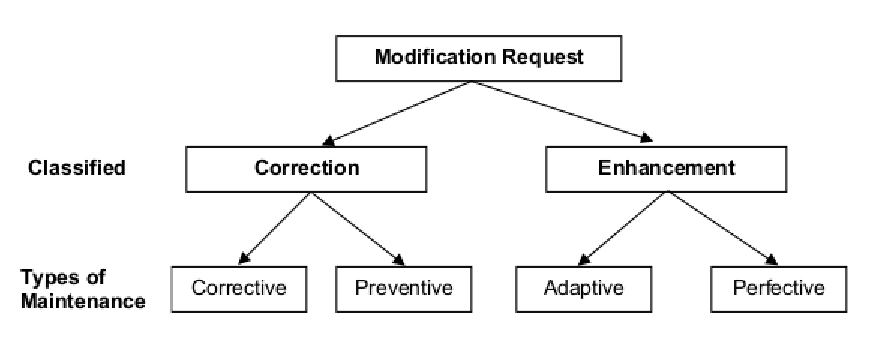
\includegraphics[width=.75\textwidth]{chapter-intro/img/modification_request.eps}
\caption{Tipos de manutenção segundo a norma ISO/IEC 14764. Extraído de
  \cite{1703974}}
\label{fig:modification-request}
\end{figure}

A ISO/IEC 14764 classifica as manutenções adaptativas e perfectivas como melhorias e agrupa as
manutenções corretivas e preventidas em uma categoria de correção, conforme exibido na
Tabela~\ref{tab:categorias_requisicao_mudanca}. A manutenção preventiva é mais frequentemente
realizada em produtos de software onde a seguranças é crítica. At Modification requests are logged and tracked, the impact of proposed changes is determined, code and other software artifacts are modified, testing is conducted, and a new version of the software product is released

\begin{table}[htpb]

	\centering
	\caption{Categorias da Requisição de Mudanças. Adaptado de SWEBOK~\cite{4425813}}
	\label{tab:categorias_requisicao_mudanca}
	\begin{tabular}{l|l|l|}
		\cline{2-3}
	 & \textbf{Correção} & \textbf{Melhoria} \\ \hline
	 \multicolumn{1}{|l|}{\textbf{Próativa}} & Preventiva & Perfectiva \\ \hline
	 \multicolumn{1}{|l|}{\textbf{Reativa}} & Corretiva & Adaptativa \\ \hline
	\end{tabular}
 \end{table} 

Apesar das diferentes nomenclaturas existentes na literatura (demanda, bug, defeito, bilhete (ticket),
Requisição de Modificação, Relato de Problema) uma Requisição de Mudança representa o relato,
independente de sua estrutura, que têm por objetivo gerar uma manutenção ou evolução de um produto
de software. 
 
 \section{O processo de Manutenção de Software}
\label{sec:o_processo_de_manutecao_de_software}

Um Processo de Software é o conjunto de atividades, métodos, práticas e transformações no qual
pessoas utilizam para desenvolver e manter software e seus artefados associados~\cite{paulk1993key}. The Maintenance Process subarea provides references and standards used to implement the software
maintenance process.
\subsection{Manutenção de Software Tradicional}
\label{subsec:manutenção_de_software_tradicional}
Maintenance processes provide needed activities and
detailed inputs/outputs to those activities, and are described in software maintenance standards
IEEE 1219 and ISO/IEC 14764.
The maintenance process model described in the Standard for Software Maintenance (IEEE1219) starts
with the software maintenance effort during the post-delivery stage and discusses items such as
planning for maintenance. That process is depicted in Figure 2.

SO/IEC 14764 [ISO14764-99]
is an elaboration of the
IEEE/EIA 12207.0-96 maintenance process. The activities of the ISO/IEC maintenance process are
similar to those of the IEEE, except that they are aggregated a little differently. The maintenance
process activities developed by ISO/IEC are shown in Figure 3.

Each of the ISO/IEC 14764 primary software maintenance activities is further broken down into tasks,
as follows.

?Process Implementation ? Problem and Modification Analysis ? Modification Implementation ?
Maintenance Review/Acceptance ? Migration ? Software Retirement

As already noted, many maintenance activities are similar to those of software development.
Maintainers perform analysis, design, coding, testing, and documentation. They must track
requirements in their activities just as is done in development, and update
documentation as
baselines
change.

ntainers and rerouted to a developer
[Dor02],
(Apr01)
? Modification Request and Problem Report Help Desk: an end-user support function that triggers the
assessment, prioritization, and costing
of
modification requests [Ben00]
? Impact Analysis (see section 2.1.3 for details) ? Software Support: help
and advice to users
concerning a request for information (for example, business rules, validation, data meaning and
ad-hoc requests/reports) (Apr03)
? Service Level Agreements (SLAs) and specialized (domain-specific) maintenance contracts which are
the responsibility of the maintainers (Apr01)


Assess the risk of a given release and develop a back-out plan in case problems should arise
? Inform all the stakeholders

\subsection{Manutenção de Software com Método dos Agilistas}
\label{sub:manutenção_de_software_com_método_dos_agilistas}

Recently, agile methodologies have been emerging which promote light processes. This requirement
emerges from the ever- increasing demand for
fast turn-around of maintenance
services. Some experiments with Extreme maintenance are presented in

\section{Ferramentas de Gerenciamento de Requisições de Mudança (FGRM)}
\label{sec:ferramentas_de_gerenciameto_de_requisições_de_mudança}

\subsection{Características Gerais}
\label{subsec:caracteristicas_gerais}

\subsection{Extensões para FGRM}
\label{subsec:extensoes_para_fgrm}







